\section{Neural Network}
\label{model:mlp}
We first discuss the early neural network, perceptron. The function takes a $d$-dimension vector $\mathbf{x}$ as input along with a weight vector $\mathbf{w}$ and calculates a single output. 
\begin{align} \label{eqn: perceptron}
    a = f(\mathbf{x}) = \sigma(\mathbf{w}^T\mathbf{x} + b)
\end{align}
where $\mathbf{w}^T\mathbf{x} = \sum_{i=0}^{d} \omega_{i}x_{i} $ denotes the inner product between the input and weight vector and $b$ is bias. The perceptron behaves as a nonlinear function $\sigma$ of a linear combination of the input where each element $x_{i}$ is multiplied with it's corresponding coefficient $\omega_{i}$. 
Figure ... illustrates the process of a single perceptron process.\\
At first, the perceptron function is designed to solve the \textit{binary classification} problem in which each datapoint $\mathbf{x}$ belongs to a single class (denoted as \textbf{1} or \textbf{0}) and the weight vector $\mathbf{w}$ represents a boundary hyperplane that splits the space into two classes seperately. 
Therefore, points that lie at the same side of the plane are grouped to the same class. 
And the $sign$ function is used as activation function $\sigma$ in \ref{eqn: perceptron} to return $1$ if the combination is positive and $0$ otherwise.
\begin{align} \label{eqn: sgn_perceptron}
    a = f(\mathbf{x}) = \left\{\begin{matrix}
1 & \text{\quad if \quad} \mathbf{w}^T\mathbf{x} + b\geq 0 \\ 
0 & \text{\quad if \quad} \mathbf{w}^T\mathbf{x} + b <  0 
\end{matrix}\right.
\end{align}

Neural network is a combination of a large number of interconnected processing elements (called \textit{neuron}) organized in a multi-layer architecture, where signal from a neuron can be passed to another from nearby layers (figure ...).
Each neuron is also formulated the same form as \ref{eqn: perceptron}. 
In general, neural network has an input layer, an output layer and a predefined number of hidden layers. 
Each hidden layer stands for a single transformation step in the process, which aims to extract hidden patterns of the input stored in it's neurons. These information is continually passed to following layers to extract more essential features. 
Due to the fact that sequence of linear transformations always equals to a single linear one, neural network uses nonlinear activation function $\sigma$ to element-wise apply to each processed neuron. 
Different from perceptron, activation function here is continuous, which makes the network weights differentiable with respect to output signals. \\
\begin{figure}[t!]
    \centering
    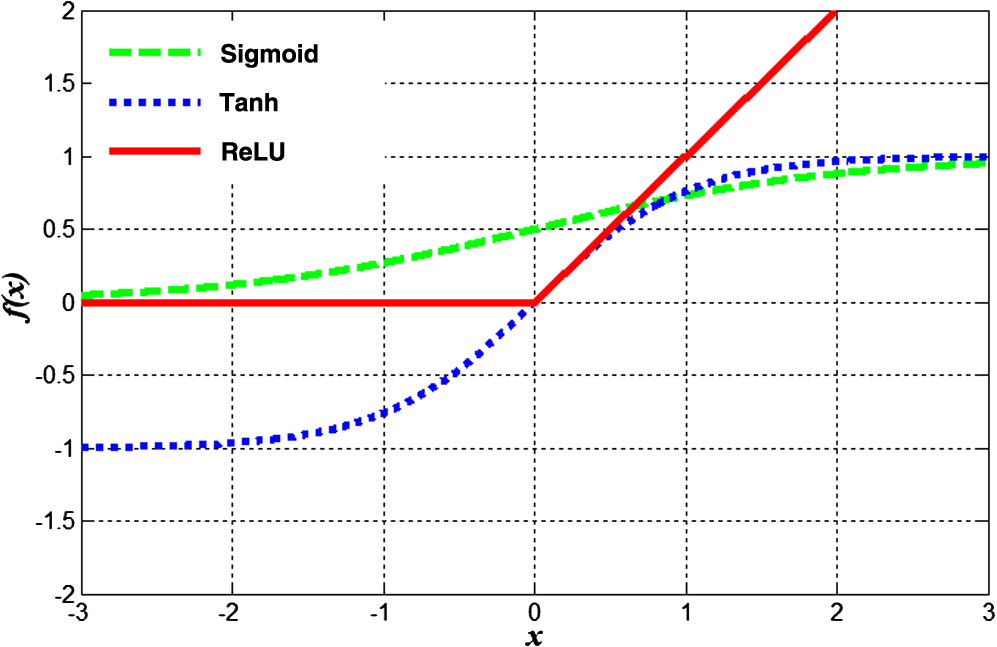
\includegraphics[width=0.7\textwidth]{resources/images/activation.png}
    \caption{Plot of Sigmoid, Tanh and ReLU activation functions.}
    \label{fig:activation}
\end{figure}
Here we list some of those activation functions commonly used in neural network modeling:
\begin{align} \label{eqn:sigmoid}
    \mathrm{sigmoid}(x) = \frac{1}{1 + \exp(-x)}
\end{align}
\begin{align} \label{eqn:tanh}
    \mathrm{tanh}(x) = \frac{\exp(2x - 1)}{\exp(2x + 1)} = 2 \times \mathrm{sigmoid}(2x) - 1
\end{align}
\begin{align} \label{eqn:relu}
    \mathrm{relu}(x) = \mathrm{max}(0, x)
\end{align}
The $sigmoid$ function (\ref{eqn:sigmoid}) scales real numbers to the range $[0, 1]$, where the large positive numbers change to $1$ and the large negative ones become $0$. Similar to $sigmoid$ but aims to produce zero-centered signals, $tanh$ function (\ref{eqn:tanh}) is a scaled version of $sigmoid$ with values range of $[-1, 1]$.\\
The drawback of both $sigmoid$ and $tanh$ is that when the numbers are large, the squashed values are saturated, hence their gradients is extremely small, which leads to the vanish problem when training deep neural networks. In such cases, Rectified Linear Unit ($ReLU$, \ref{eqn:relu}) is preferably used, which converts negative values to zero while keep the positive ones.
Figure \ref{fig:activation} illustrates the three functions in the same input range.


